\fbckg{background/recoleccion_de_datos}
\begin{frame}
    \Huge
    \misc{
        Recolección de datos
    }
\end{frame}

\fbckg{background/CDMX}
\begin{frame}
    \Huge
    \misc{
        Mediciones in situ
    }
\end{frame}

\fbckg{background/white}
\begin{frame}
    \misc{
        \begin{minipage}{0.48\linewidth}
            \begin{figure}[H]
                \centering
                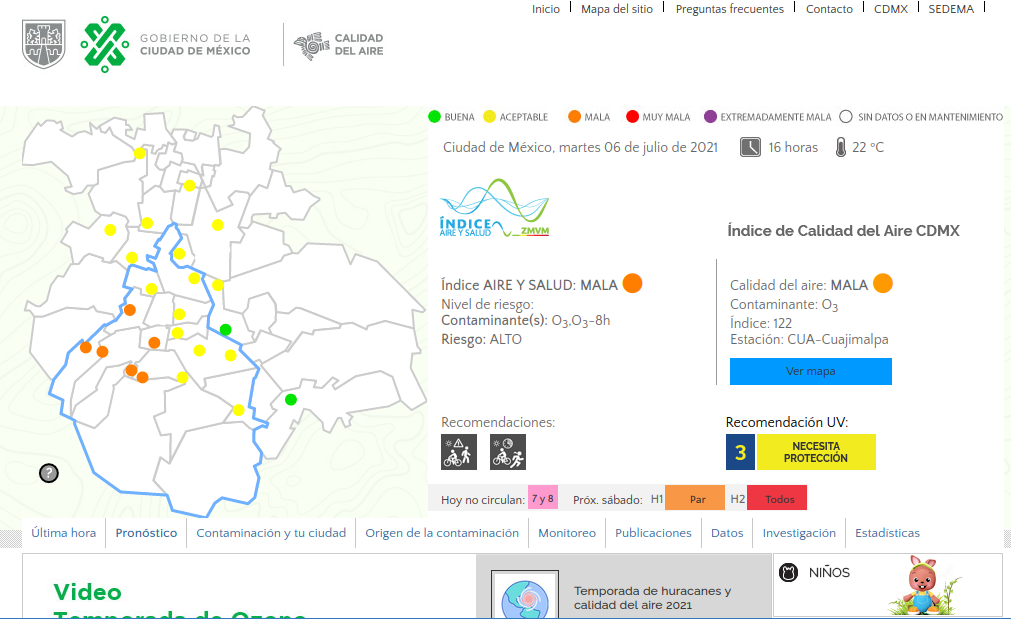
\includegraphics[height=4.5cm,width=6.2cm]{sedema_web}
                \caption{Página web de la SEDEMA. \cite{SEDEMA_page}}
            \end{figure}
        \end{minipage}
        \begin{minipage}{0.48\linewidth}
            \begin{figure}[H]
                \centering
                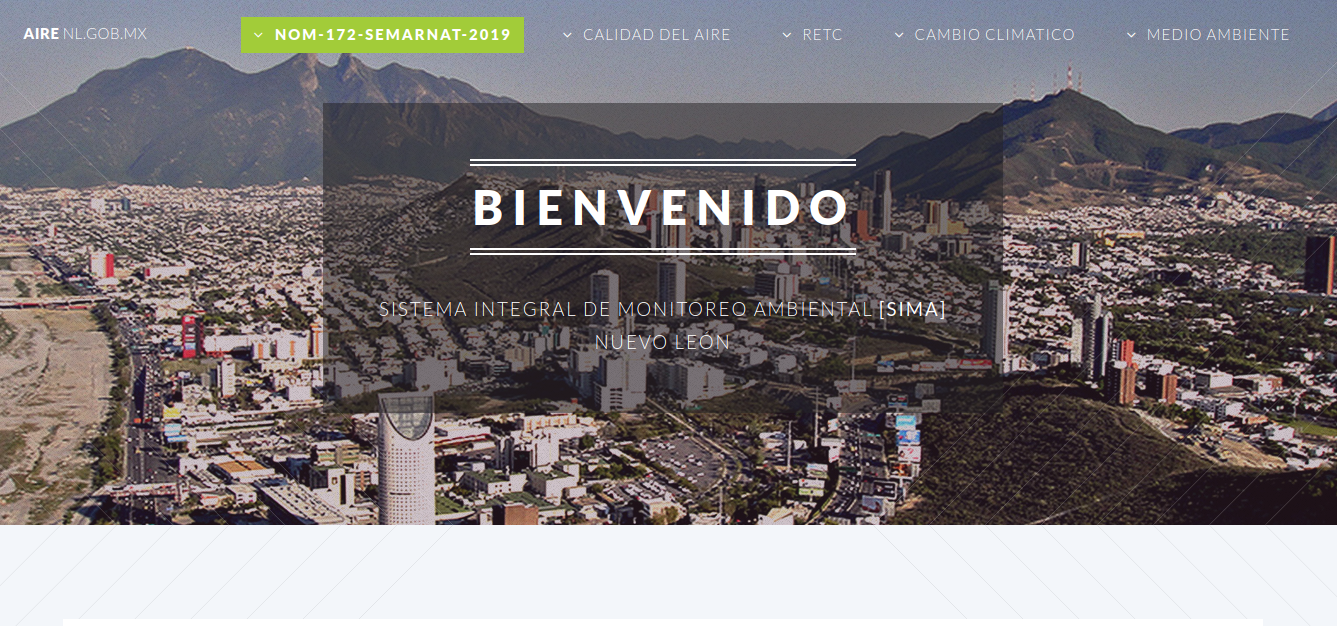
\includegraphics[height=4.5cm,width=6.2cm]{sima_web}
                \caption{Página web del SIMA. \cite{SIMA_page}}
            \end{figure}
        \end{minipage}
    }
\end{frame}

\begin{frame}
    \Huge
    \misc{
        \begin{align*}
            \text{UVB}     & \rightarrow [280nm,320nm] \\
            \text{UVA}     & \rightarrow [320nm,400nm] \\
            \text{UVB+UVA} & \rightarrow [280nm,400nm] \\
        \end{align*}
    }
\end{frame}

\begin{frame}
    \renewcommand{\yourowntexcol}{black}
    \begin{figure}[H]
        \centering
        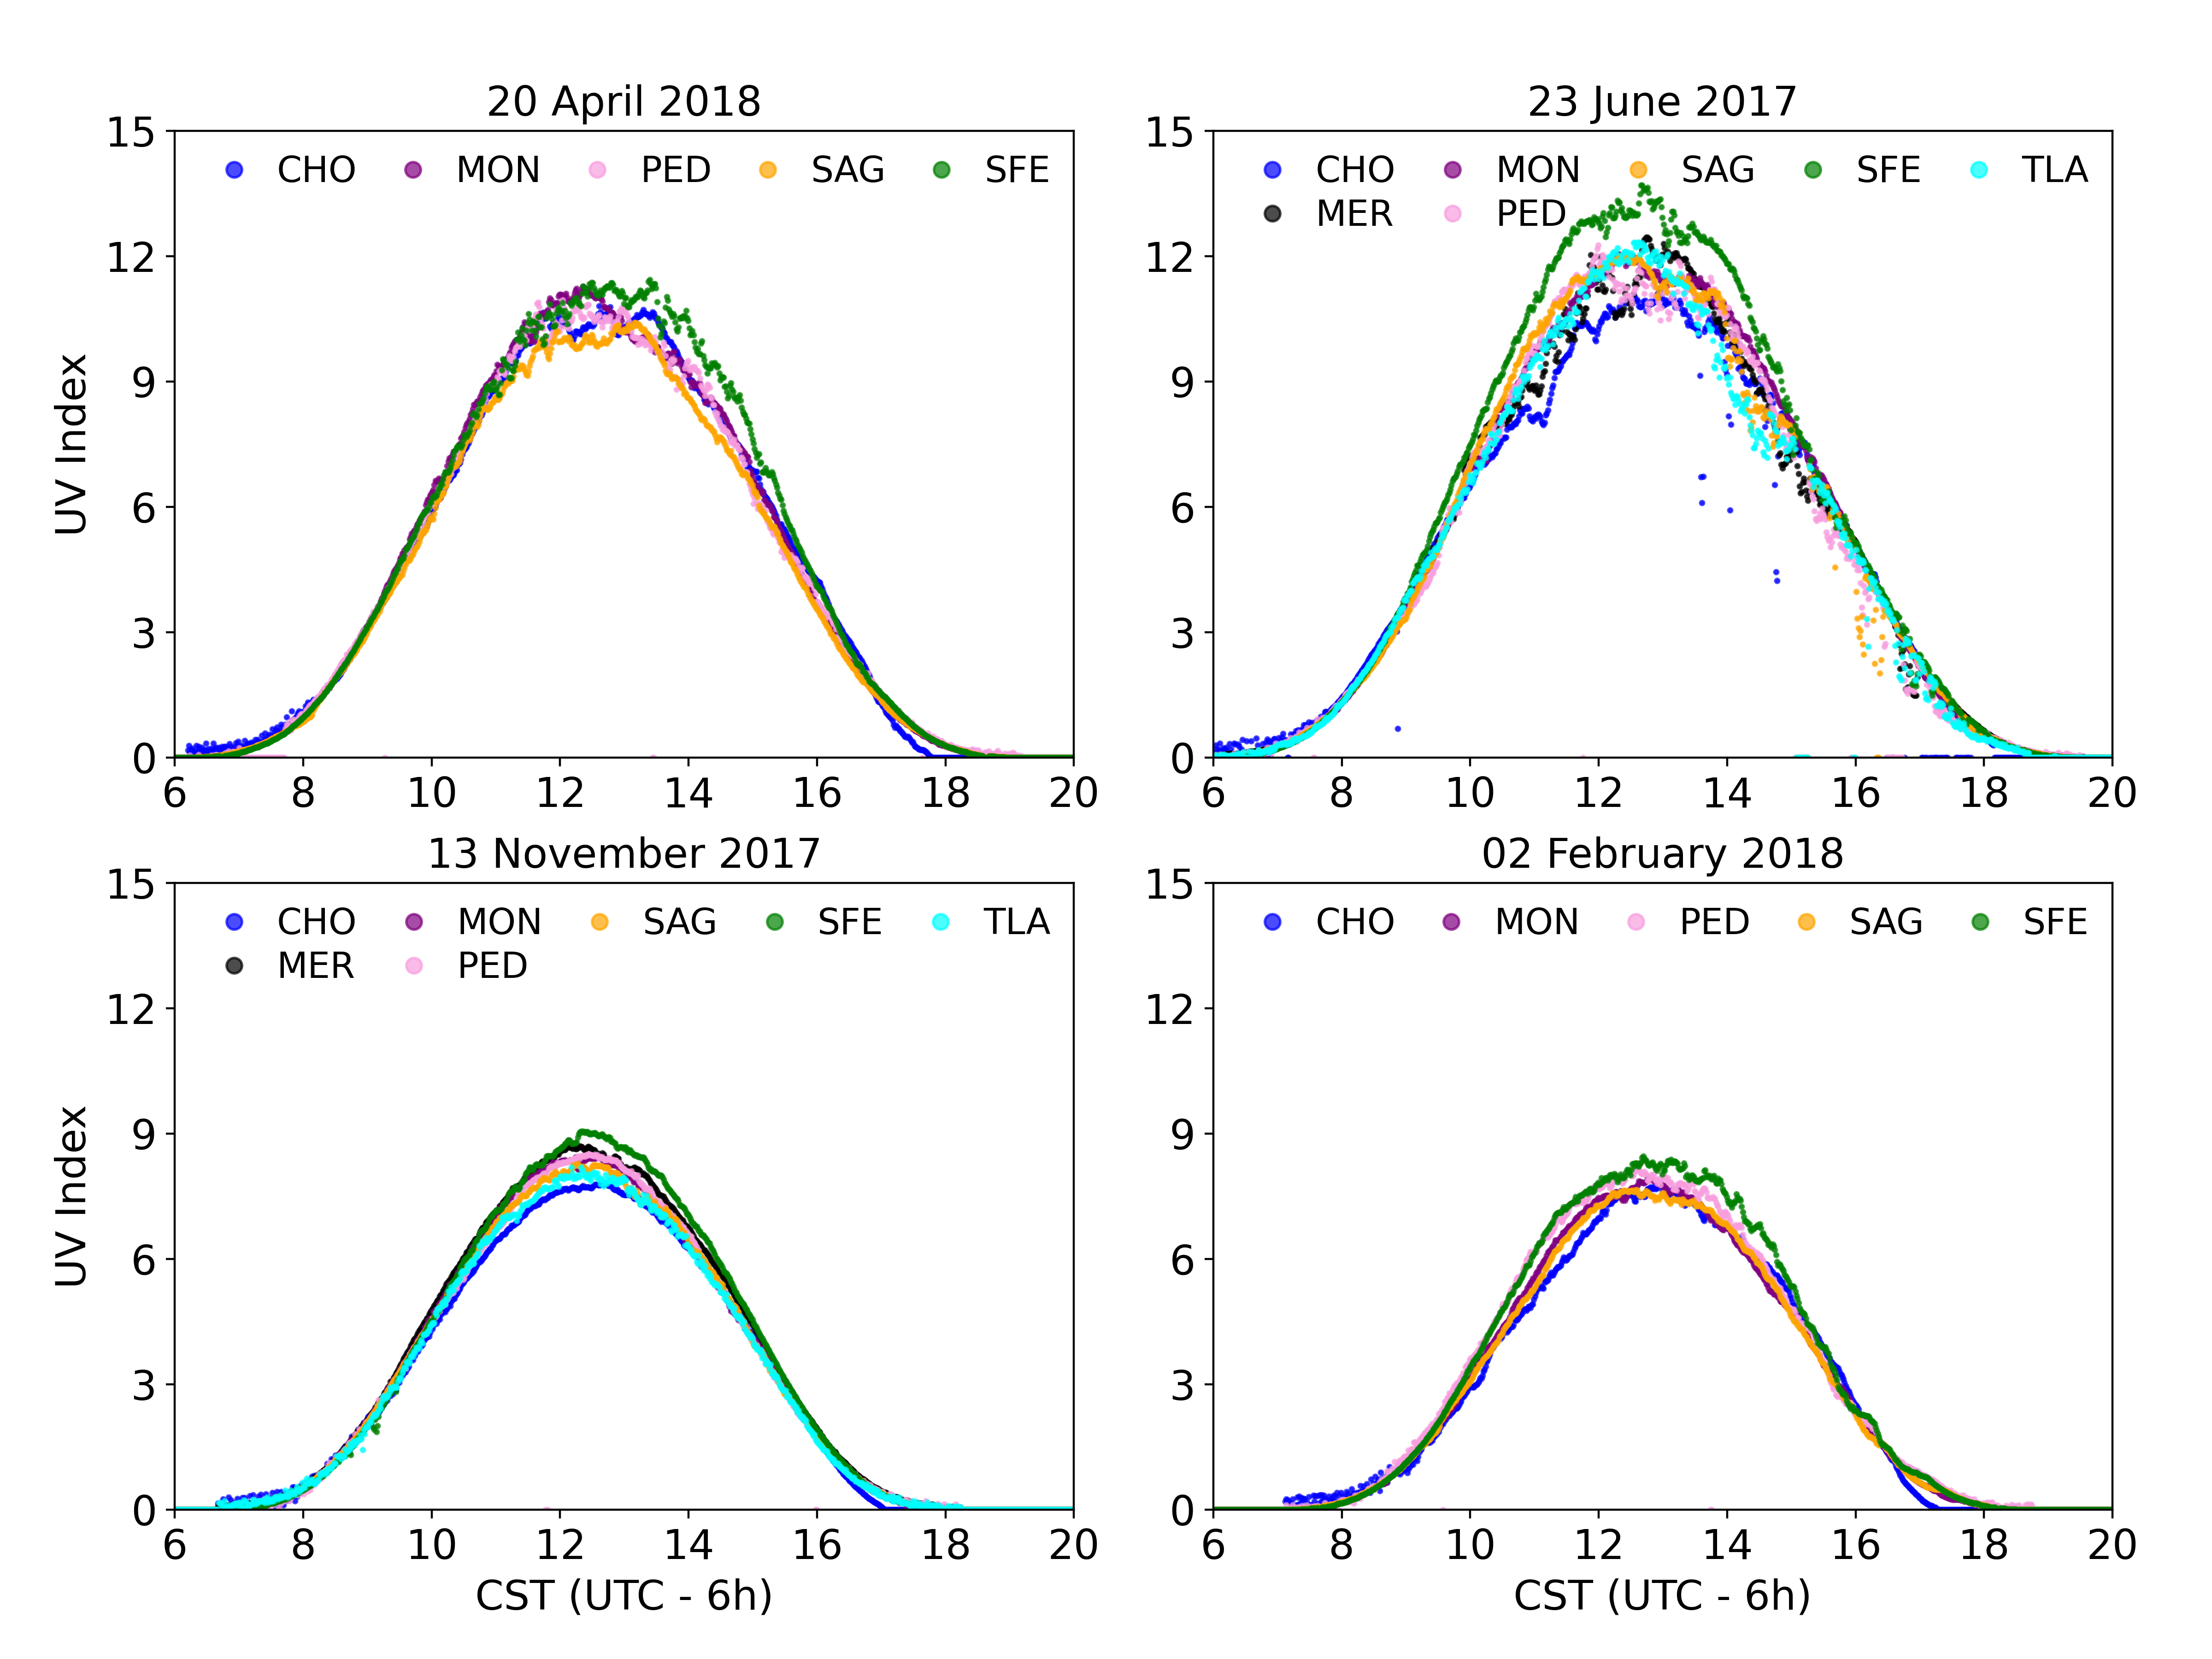
\includegraphics[width=9cm,height=7cm]{season.png}
        \caption{Mediciones de indice UV en las diferentes estaciones de monitoreo de la SEDEMA. \cite{SEDEMA_page}}
    \end{figure}
\end{frame}

\fbckg{background/aura_satelite}
\begin{frame}
    \Huge
    \misc{
        Mediciones satelitales
    }
\end{frame}

\fbckg{background/white}
\begin{frame}
    \misc{
        \begin{minipage}{0.48\linewidth}
            \begin{figure}[H]
                \centering
                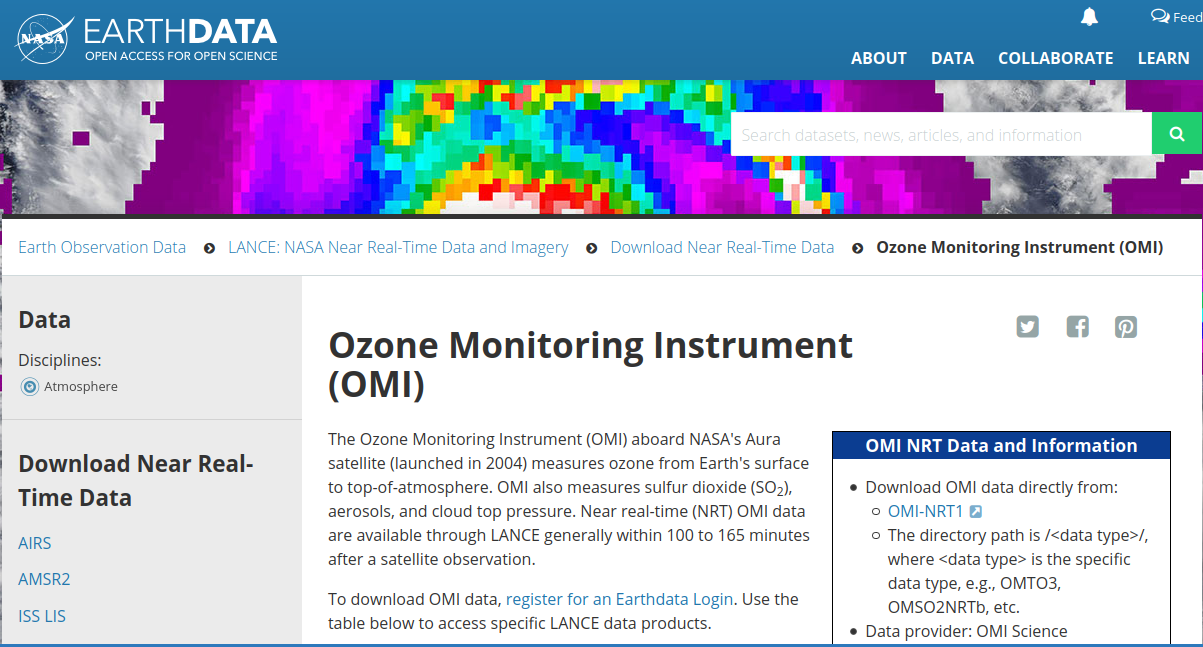
\includegraphics[width=6.2cm,height=5cm]{OMI_web}
                \caption{Página web del proyecto OMI. \cite{OMI_page}}
            \end{figure}
        \end{minipage}
        \begin{minipage}{0.5\linewidth}
            \begin{figure}[H]
                \centering
                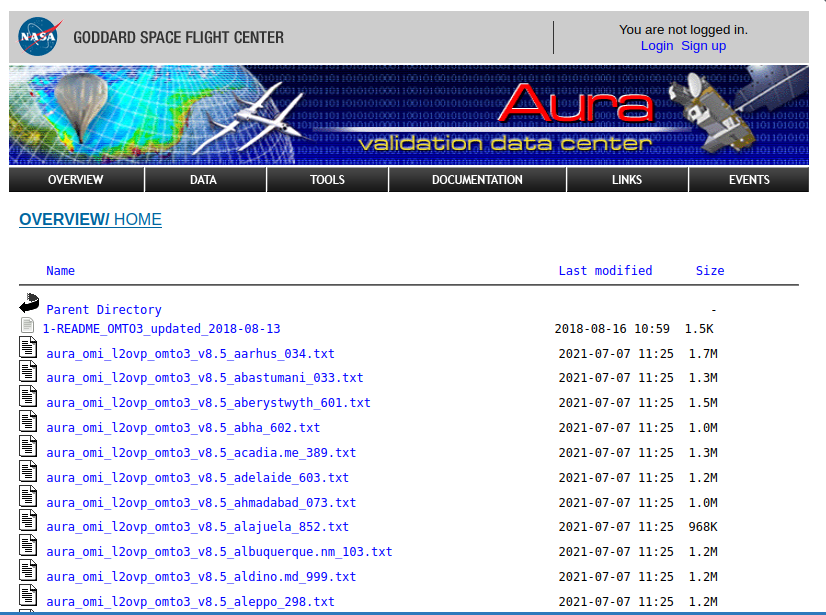
\includegraphics[width=6.2cm,height=5cm]{data_web}
                \caption{Página web de los datos OMI. \cite{Aura_page}}
            \end{figure}
        \end{minipage}
    }
\end{frame}

\begin{frame}
    \renewcommand{\yourowntexcol}{black}
    \begin{minipage}{0.45\linewidth}
        \begin{figure}[H]
            \centering
            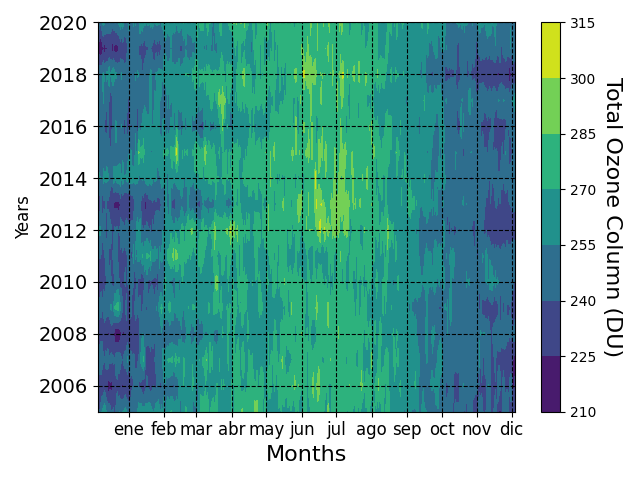
\includegraphics[width=6.2cm,height=5cm]{ozone_cdmx}
            \caption{Datos de columnas de Ozono en CDMX.}
        \end{figure}
    \end{minipage}
    \hspace{0.5cm}
    \begin{minipage}{0.45\linewidth}
        \begin{figure}[H]
            \centering
            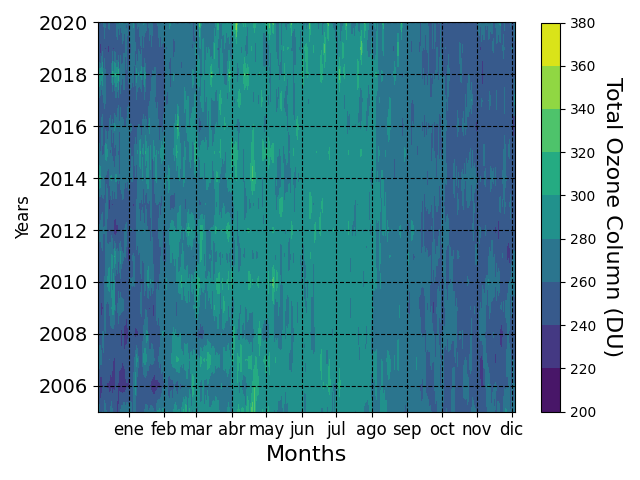
\includegraphics[width=6.2cm,height=5cm]{ozone_mty}
            \caption{Datos de columnas de Ozono en Monterrey.}
        \end{figure}
    \end{minipage}
\end{frame}